\documentclass[tikz,border=3mm]{standalone}
\usepackage[T1]{fontenc}
\usepackage{lmodern,amsmath,amssymb}
\usetikzlibrary{arrows.meta,calc,positioning,fit,backgrounds}
\definecolor{accent}{RGB}{36,91,158}
\definecolor{soft}{RGB}{225,237,248}
\definecolor{muted}{RGB}{122,134,145}
\definecolor{warm}{RGB}{250,242,220}
\tikzset{every node/.style={font=\sffamily\small},
vertex/.style={circle,draw=black!80,fill=white,minimum size=7.5mm,inner sep=1pt},
edge/.style={draw=accent!55,line width=.65pt},
highlight/.style={draw=accent,line width=1.7pt},
box/.style={draw=accent!70,rounded corners=2pt,fill=soft!45,align=center,inner sep=6pt},
heading/.style={font=\sffamily\bfseries\normalsize,align=center},
map/.style={-{Stealth[length=2mm]},line width=.8pt},
}
\hyphenpenalty=10000\exhyphenpenalty=10000
\begin{document}
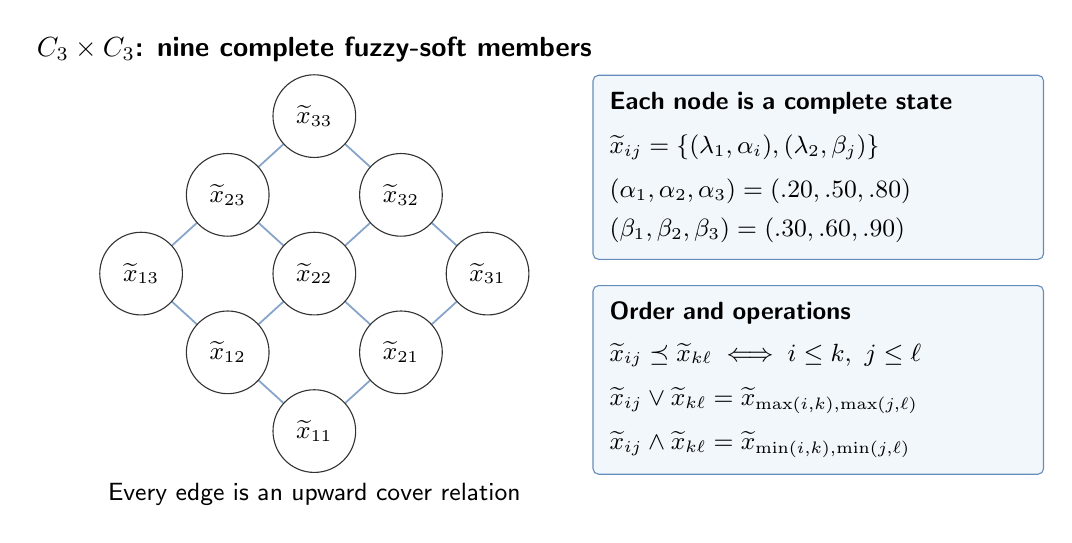
\begin{tikzpicture}[x=1cm,y=1cm]
\coordinate (xp11) at (0.000,0.000);
\coordinate (xp12) at (-1.100,1.000);
\coordinate (xp13) at (-2.200,2.000);
\coordinate (xp21) at (1.100,1.000);
\coordinate (xp22) at (0.000,2.000);
\coordinate (xp23) at (-1.100,3.000);
\coordinate (xp31) at (2.200,2.000);
\coordinate (xp32) at (1.100,3.000);
\coordinate (xp33) at (0.000,4.000);
\draw[edge] (xp11) -- (xp21);
\draw[edge] (xp11) -- (xp12);
\draw[edge] (xp12) -- (xp22);
\draw[edge] (xp12) -- (xp13);
\draw[edge] (xp13) -- (xp23);
\draw[edge] (xp21) -- (xp31);
\draw[edge] (xp21) -- (xp22);
\draw[edge] (xp22) -- (xp32);
\draw[edge] (xp22) -- (xp23);
\draw[edge] (xp23) -- (xp33);
\draw[edge] (xp31) -- (xp32);
\draw[edge] (xp32) -- (xp33);
\node[vertex,minimum size=10.5mm] (x11) at (xp11) {$\widetilde{x}_{11}$};
\node[vertex,minimum size=10.5mm] (x12) at (xp12) {$\widetilde{x}_{12}$};
\node[vertex,minimum size=10.5mm] (x13) at (xp13) {$\widetilde{x}_{13}$};
\node[vertex,minimum size=10.5mm] (x21) at (xp21) {$\widetilde{x}_{21}$};
\node[vertex,minimum size=10.5mm] (x22) at (xp22) {$\widetilde{x}_{22}$};
\node[vertex,minimum size=10.5mm] (x23) at (xp23) {$\widetilde{x}_{23}$};
\node[vertex,minimum size=10.5mm] (x31) at (xp31) {$\widetilde{x}_{31}$};
\node[vertex,minimum size=10.5mm] (x32) at (xp32) {$\widetilde{x}_{32}$};
\node[vertex,minimum size=10.5mm] (x33) at (xp33) {$\widetilde{x}_{33}$};
\node[heading] at (0,4.85) {$C_3\times C_3$: nine complete fuzzy-soft members};
\node[box,text width=5.3cm,align=left] at (6.4,3.35) {\textbf{Each node is a complete state}\\[5pt]
$\widetilde{x}_{ij}=\{(\lambda_1,\alpha_i),(\lambda_2,\beta_j)\}$\\[5pt]
$(\alpha_1,\alpha_2,\alpha_3)=(.20,.50,.80)$\\[3pt]
$(\beta_1,\beta_2,\beta_3)=(.30,.60,.90)$};
\node[box,text width=5.3cm,align=left] at (6.4,.65) {\textbf{Order and operations}\\[4pt]
$\widetilde{x}_{ij}\preceq\widetilde{x}_{k\ell}\iff i\le k,\ j\le\ell$\\[5pt]
$\widetilde{x}_{ij}\vee\widetilde{x}_{k\ell}=\widetilde{x}_{\max(i,k),\max(j,\ell)}$\\[5pt]
$\widetilde{x}_{ij}\wedge\widetilde{x}_{k\ell}=\widetilde{x}_{\min(i,k),\min(j,\ell)}$};
\node[align=center] at (0,-.8) {Every edge is an upward cover relation};
\end{tikzpicture}
\end{document}
